
\subsection{Analysis of Critical Time}


When the simplified and the extended models of the IEEE benchmark are compared for the estimation of the critical time in Figure \ref{fig:res_tcr}, it is noticed a higher deviation in the low range of RoCoF. This due to the fact that in this range of RoCoF the critical time is long enough to allow the governor response activation of the respective synchronous machines representation. Therefore it can be stated that the simplifications made in the model have a greater influence on the results for low values of penetration of IBG and low power imbalances; in this sense, the simplifications become less significant as the RoCoF increases in such a manner that the activated synchronous primary reserve is not relevant in frequency support. In the range of values of RoCoF higher than 2 Hz/s, the critical time trend for the European grid-scale and the simplified IEEE model get closer each other as RoCoF increases.\\

\begin{figure}[h]
	\centering
	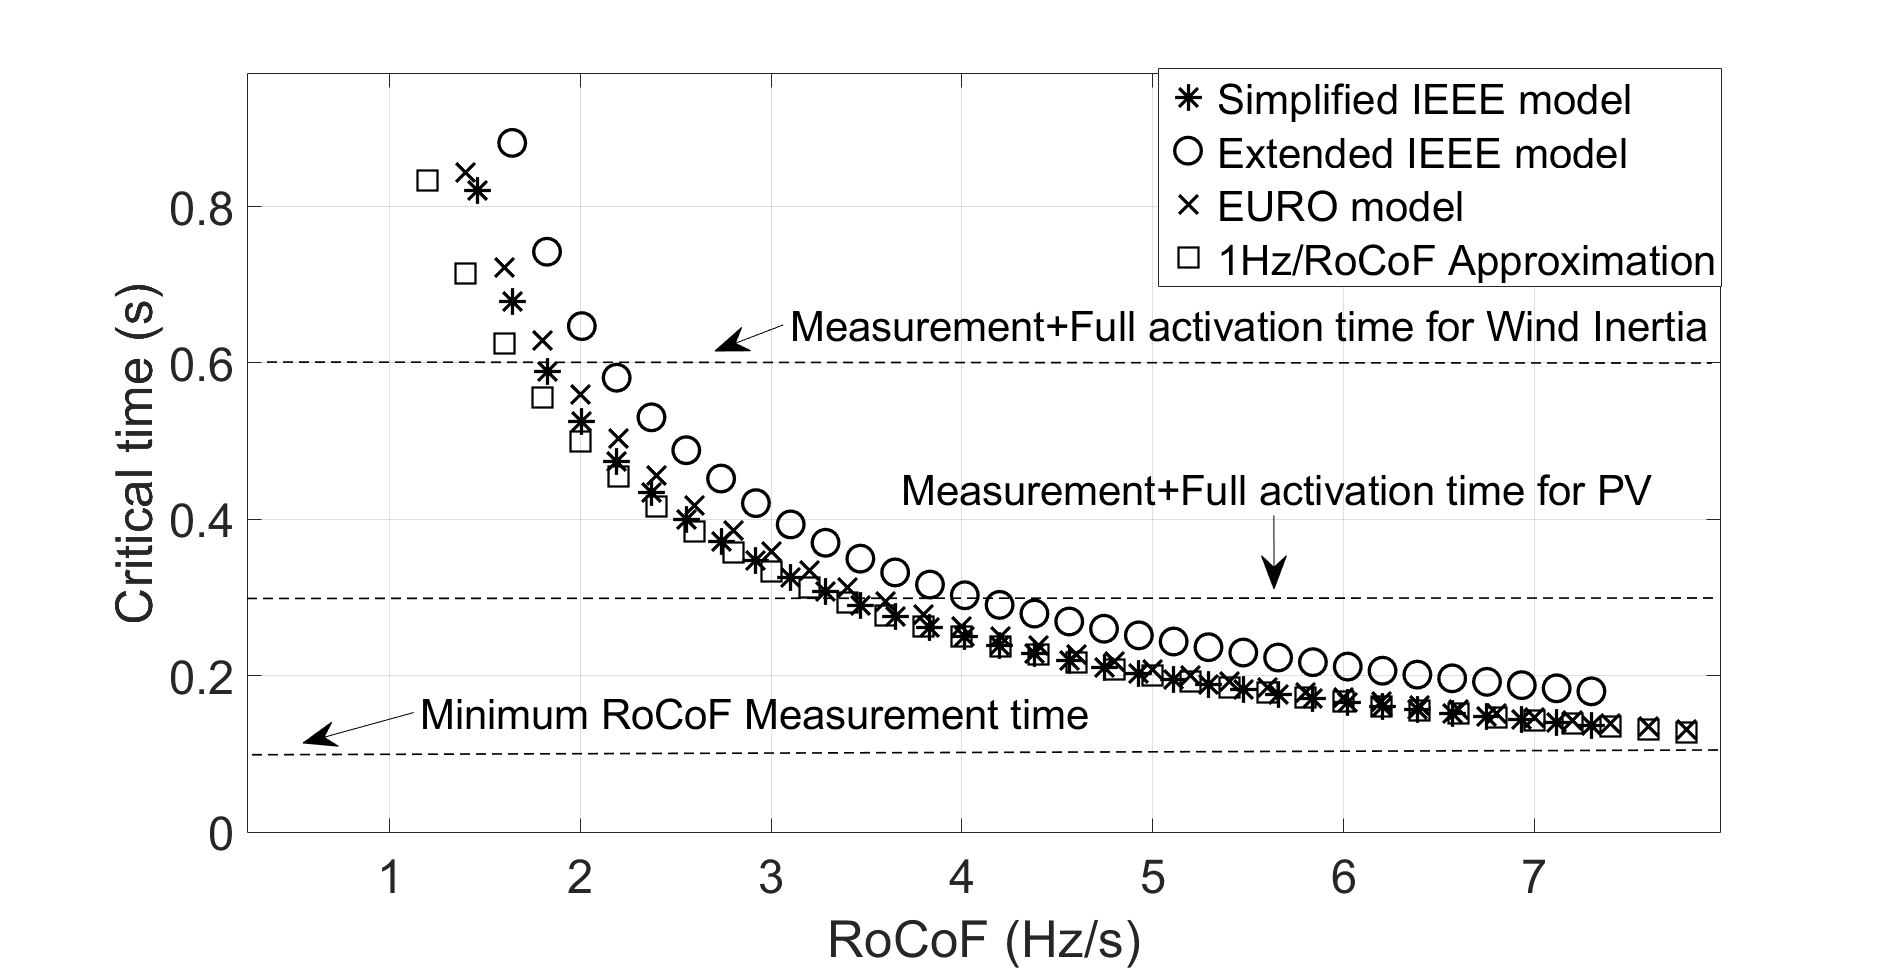
\includegraphics[width=0.75\textwidth]{/result/tcr80}
	\caption{Results for critical time in all simulated models with a penetration of IBG of 80\% .}
	\label{fig:res_tcr}
\end{figure}


Therefore under high RoCoF conditions in any of the models, the primary reserve does not significantly counteract the frequency drop [16]. Figure \ref{fig:res_tcr} demonstrates that primary reserve can be neglected for determining the critical time when the combination of IBG and load imbalances would lead to high values of RoCoF; as RoCoF increases, the approximation of critical time as 1 Hz/RoCoF narrows the difference with the results obtained from simulations [14]. Nevertheless, such simplification applies to the simplified IEEE model and the European island. Hence, the influence of all the dynamics and machine components, such as
generator exciter and damping windings, seems to improve the critical time. The damping torque in Equation \eqref{eq:swing} was not considered in the IEEE simplified model; the inclusion of such may lead to more accurate results when compared with the extended model.\\
\begin{table}[h]
	\caption{\label{tb:crtime}: Critical time for European-scale case given in seconds.}
	\centering
	%% \tablesize{} %% You can specify the fontsize here, e.g., \tablesize{\footnotesize}. If commented out \small will be used.
	\begin{tabular}{*9c}
		\toprule
		\textbf{IBG share (\%)}	& \multicolumn{8}{c}{\textbf{Load Imbalance (\%)}} \\
		\midrule
		{} & 3&	4&	5&	6&	7&	8&	9	&10 \\
		\midrule
		20&	-&	-&	6.081&	4.517&	3.629&	3.050&	2.638&	2.316\\
		40&	-&	6.226&	4.169&	3.215&	2.628&	2.222&	1.934&	1.705\\
		60	&7.142&	3.639&	2.623&	2.062&	1.698&	1.451&	1.263&	1.122\\
		80&	2.753&	1.744&	1.277&	1.018&	0.843&	0.722&	0.628&	0.559\\
		92&	1.109&	0.700&	0.514&	0.406&	0.338&	0.288&	0.252&	0.224\\
		95&	0.697&	0.436&	0.322&	0.254&	0.211&	0.179&	0.157&	0.140\\
		\bottomrule
	\end{tabular}
\end{table}






%Also it is then stated the need of a fast power response to avoid frequency collapse of islanded micro-grid or an electric island in the European scale.% Even assuming that power reserve can
%immediately fully activated after RoCoF reading, the 100 ms limitation is a constraint for high unbalanced islands with high penetration of IBG in the European case as demonstrated in the result section.

% As conclusion

%Additionally, the direct measurement of RoCoF in the 100 ms interval can lead to misleading readings [14]. In general, when penetration
%of IBG is higher than 90\%; for the 40\% imbalance an activation time between 30 and 50 ms would be needed to keep frequency within the allowed limits.
Due to the fact that the characteristics of the  European interconnected scenario provided by ENTSOE were assumed to be the same than the resulting islands after a severe event [REF]; the results for the large scale model can be understood as the behavior of the whole European system with bigger perturbations. The dimensioning scenario assumes a power imbalance of 3 GW, which corresponds to a 2\% of the 150 GW load [1]. If in the future a bigger dimensioning case is utilized, then synchronous response would not be enough to balance the system before load shedding occurs. Table \ref{tb:crtime} exhibits the required time when the dimensioning scenario is increased up to 10\% for different IBG penetration.



\subsection{Analysis of Synthetic Inertia and Fast Power Reserve}

\subsubsection{Effect Synthetic Inertia on Frequency}
\label{sec:res_si}
In this section the results of the implementation of synthetic inertia in the simplified IEEE model and the European model are presented. The frequency nadir for such systems without any additional power support apart from synchronous response are illustrated in Figures \ref{fig:res_nadirieee_simp} and \ref{fig:res_nadireuro}. \\

\begin{figure}[h]
	\centering
	\begin{subfigure}[h]{0.49\textwidth}
		\centering
		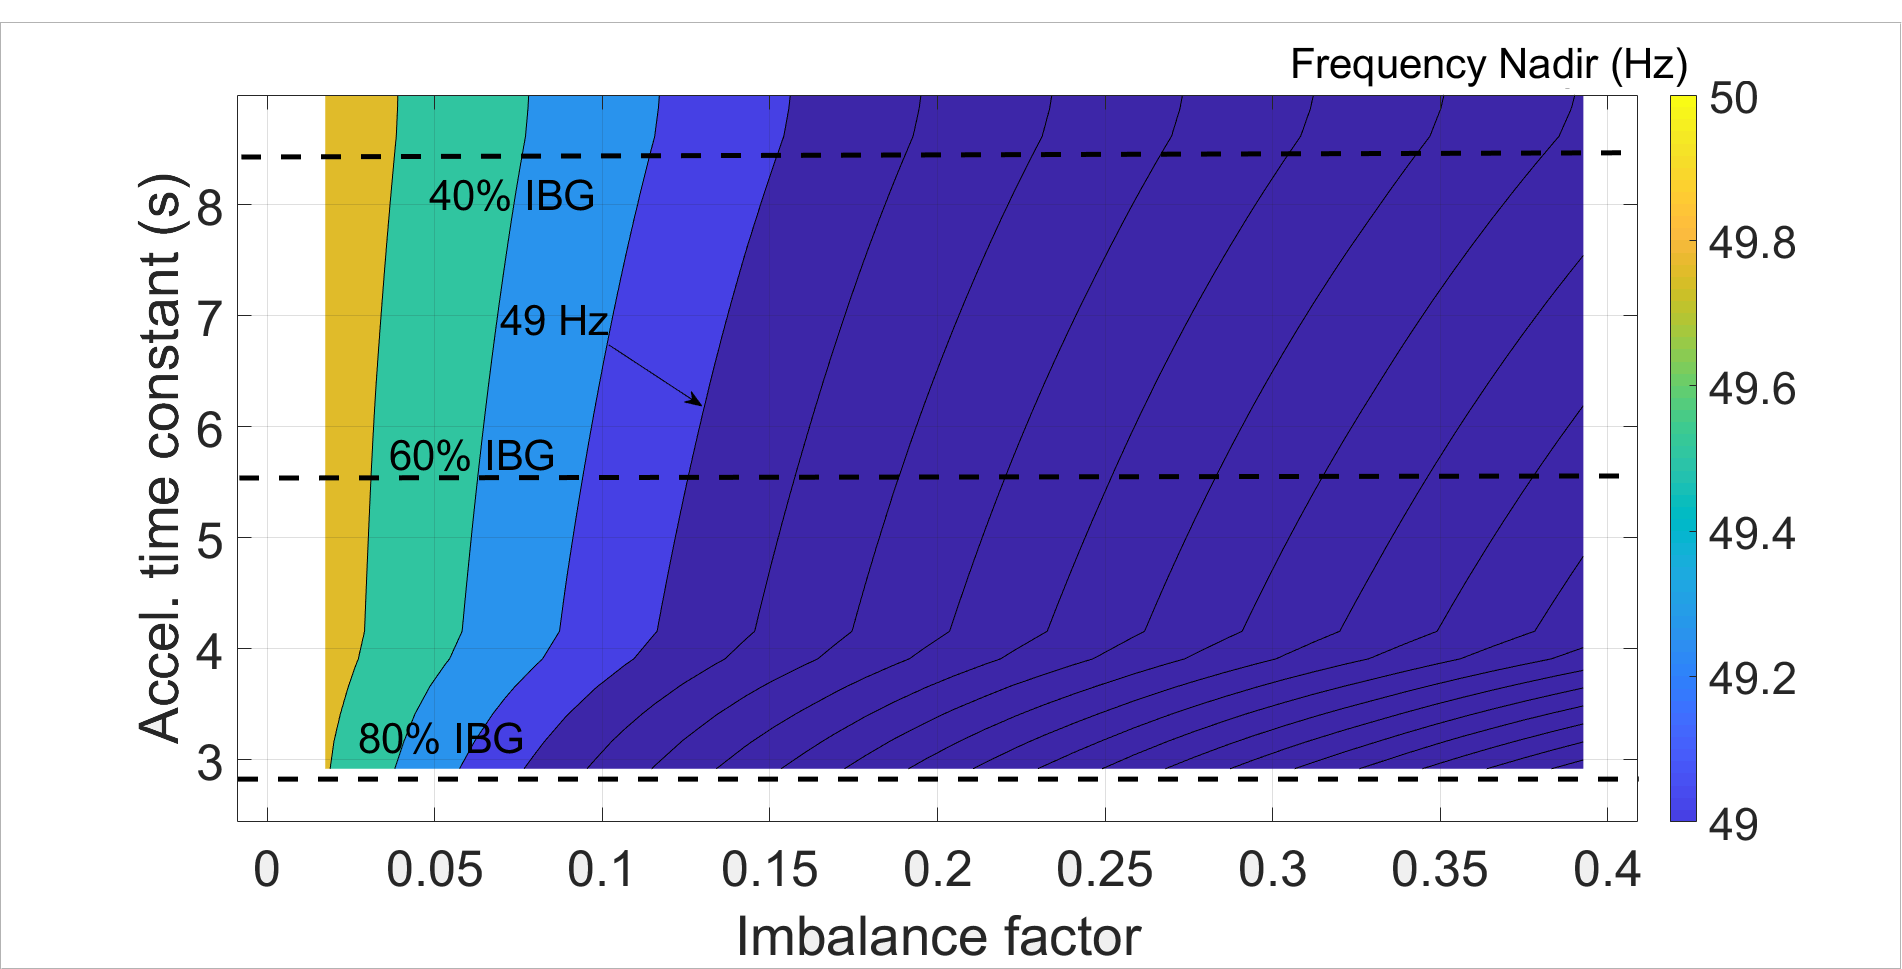
\includegraphics[width=\textwidth]{result/base}
		\caption{}
		\label{fig:res_nadirieee_simp}
	\end{subfigure}
	\hfill
	\begin{subfigure}[h]{0.49\textwidth}
		\centering
		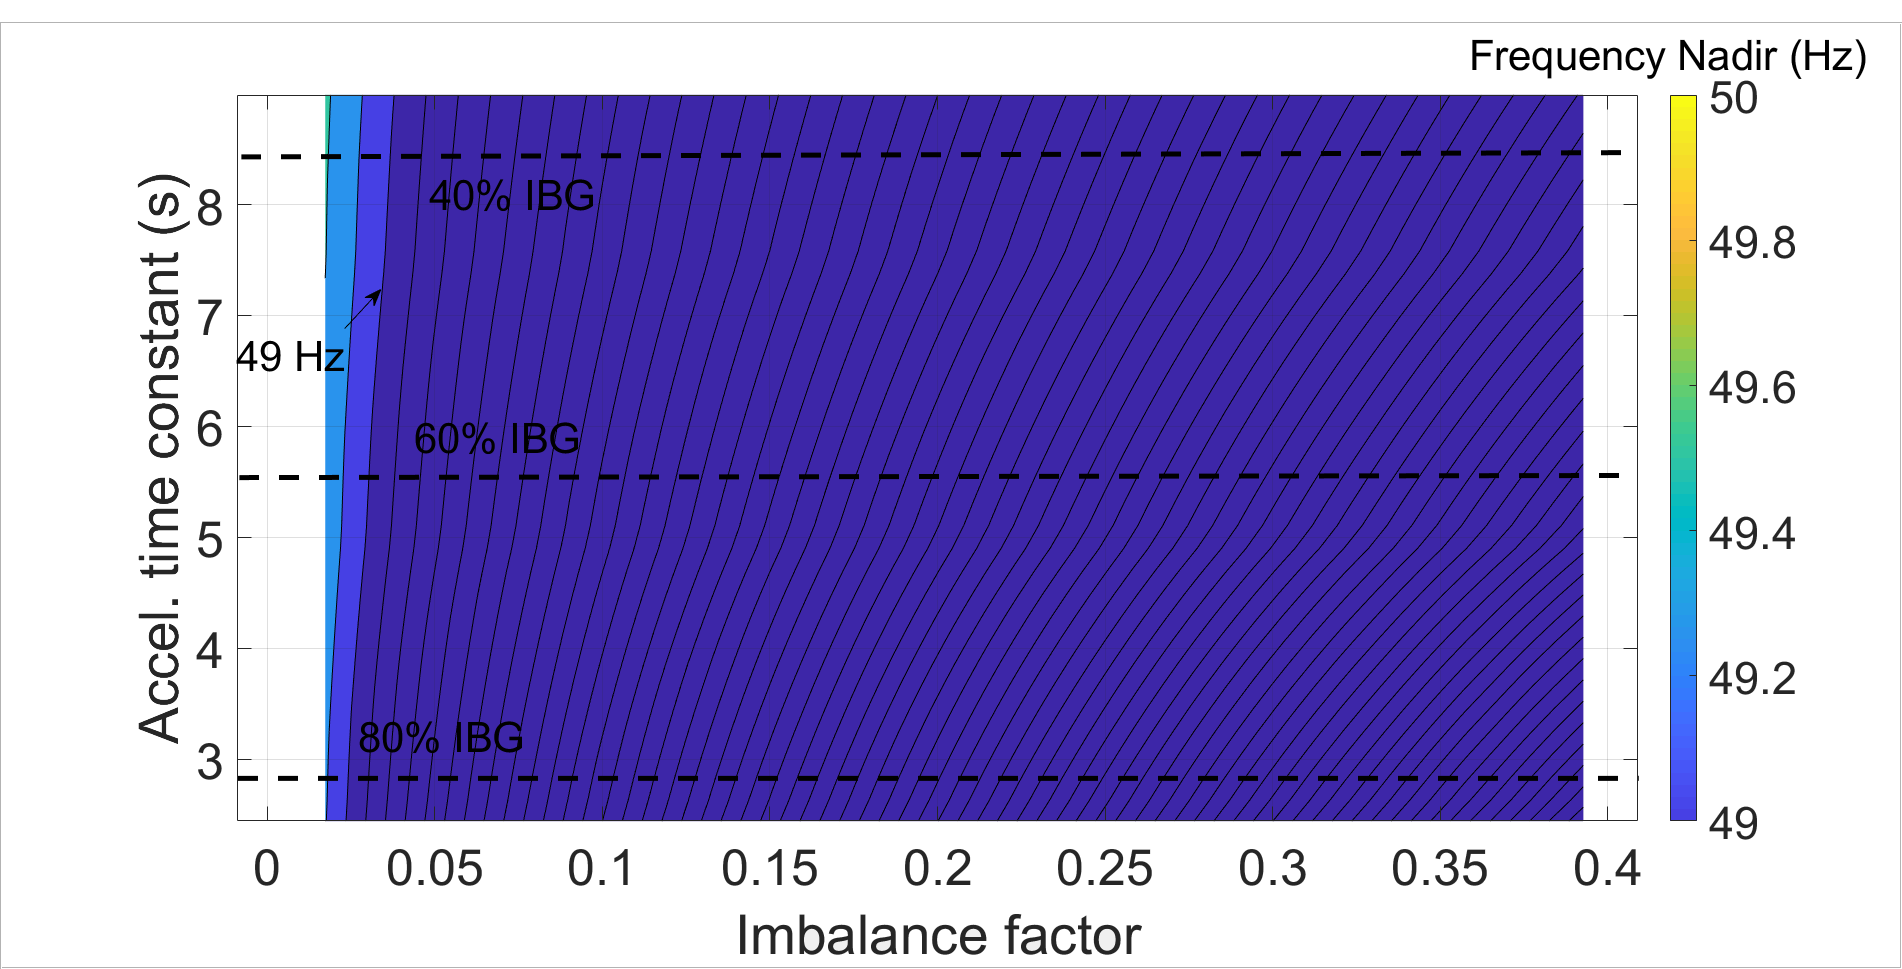
\includegraphics[width=\textwidth]{result/base_euro}
		\caption{}
		\label{fig:res_nadireuro}
	\end{subfigure}
	
	
	\caption{The frequency nadir of the simplified IEEE model is depicted in (\textbf{a}), for the acceleration constant corresponding to the 80\% of the IBG, the frequency nadir reaches values lower than 49 Hz with power imbalances starting at $ \sim 7\% $. In (\textbf{b}) the frequency nadir of the large scale-european grid is illustrated. At 80\% of IBG the frequency nadir reaches 48.73 Hz with only $\sim 3\% $ of imbalance.}
\end{figure}




In any of the cases, UFLS is not avoided for all combination of imbalances and acceleration constants with the application of synthetic inertia. It can also be observed in Figure \ref{fig:res_nadirieee_si} that values of frequency nadir under 49 Hz are reached for imbalances bigger than 14\% combined with shares of IBG above 80\% in the simplified representation of the IEEE model. Nevertheless, an enhanced performance is observed in the simplified IEEE model. The reason behind this, is the faster response of the synchronous share present in the system, which jointly performs with the synthetic inertia to improve over all frequency response performance. On the other hand, the European scale model depicted in Figure \ref{fig:res_nadireuro_si} at 80\% of IBG, reaches the value of 48.89 Hz of frequency nadir with an imbalance of 3\%. This demonstrates that synthetic inertia is not enough by itself for withstanding severe imbalances under high penetration of inverter based generators.  \\
\begin{figure}[h]
	\centering
	\begin{subfigure}[h]{0.49\textwidth}
		\centering
		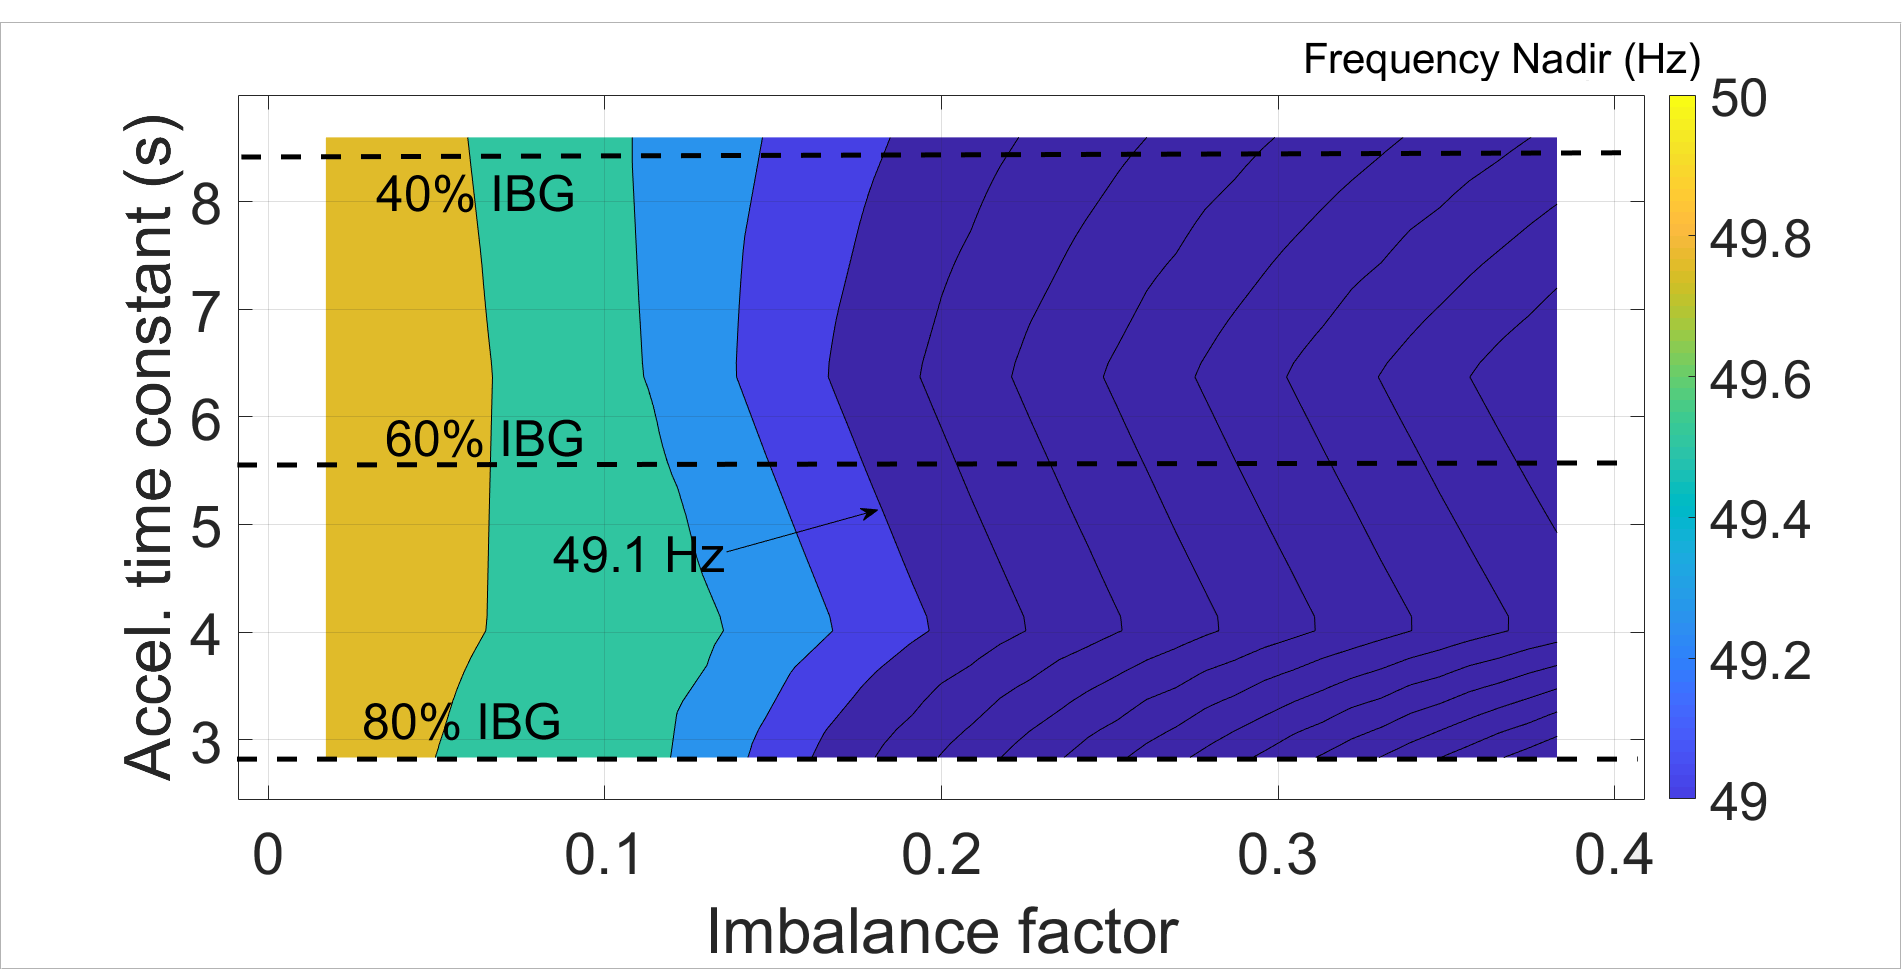
\includegraphics[width=\textwidth]{result/SI40}
		\caption{}
		\label{fig:res_nadirieee_si}
	\end{subfigure}
	\hfill
	\begin{subfigure}[h]{0.49\textwidth}
		\centering
		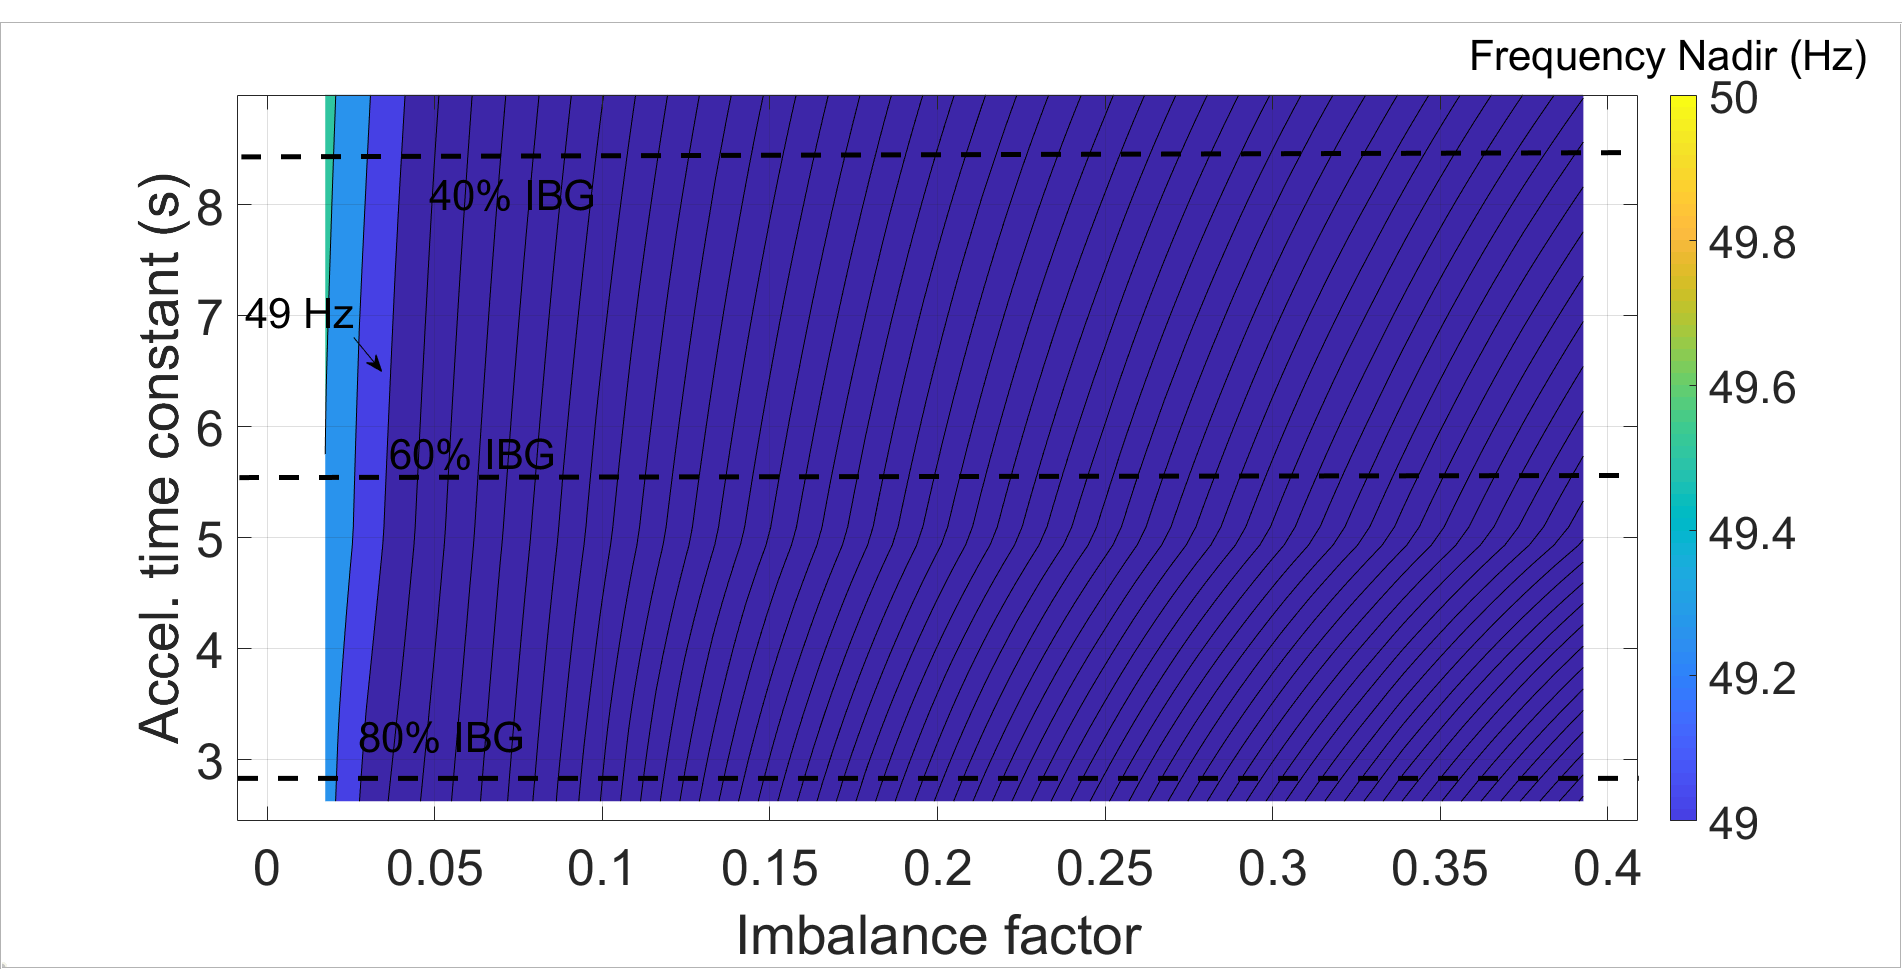
\includegraphics[width=\textwidth]{result/SI80Euro}
		\caption{}
		\label{fig:res_nadireuro_si}
	\end{subfigure}
	
	
	\caption{(\textbf{a}) Shows the frequency nadir once synthetic inertia has been applied to the 40\% of the IBG in the simplified IEEE model. (\textbf{b}) Frequency nadir of the large scale model with same share of contribution from synthetic inertia.}
\end{figure}


 %In Figure XXX can be observed how power is deployed in a few seconds in the simplified IEEE model whereas in the European model the response is always limited to fully deployment in the order of $ \sim 30 $s.



Figure \ref{fig:res_ieee_fr10imb} and \ref{fig:res_ieee_fr15imb} indicate the frequency response obtained of the system with an non-synchronous generation of 80\% for different load imbalances.  
In Figure \ref{fig:res_ieee_fr10imb} can be observed how the frequency drops below 49 Hz with a 10\% of imbalance, when no IBFPR or synthetic inertia is used as frequency support strategy. In the same figure, the frequency responses for different levels of synthetic inertia is presented. It is noticed the improvement in the response with the implementation of synthetic inertia. UFLS is avoided for every share of synthetic inertia, assuming that primary reserve takes place after synthetic inertia. As the imbalance increases, the effectiveness of the synthetic inertia decreases. Figure \ref{fig:res_ieee_fr15imb} shows how a contribution of wind power of 40\% from the inverter based generation is capable of avoiding UFLS. Nevertheless the share of 80\% begins with a low rate of frequency decrement, the frequency suddenly drops below 49 Hz. This is due to the high amount of synthetic inertia power supplying the load imbalance. This situation leads to UFLS after the 10 s because frequency has been sustained during that time by the synthetic inertia power. Since 10 seconds is the assumed time limit for exceeding nominal turbine power rate; the synthetic inertial power, which has a big contribution to counteract the power imbalance, is switched off. On the other hand, when a higher imbalance occurs and the synthetic inertia response is saturated, due to the limitation of 10\% of rated power, the mechanical power increases at 10 seconds, having a less severe impact the switching off of the inertial response.

\begin{figure}[h]
	\centering
	\begin{subfigure}[h]{0.49\textwidth}
		\centering
		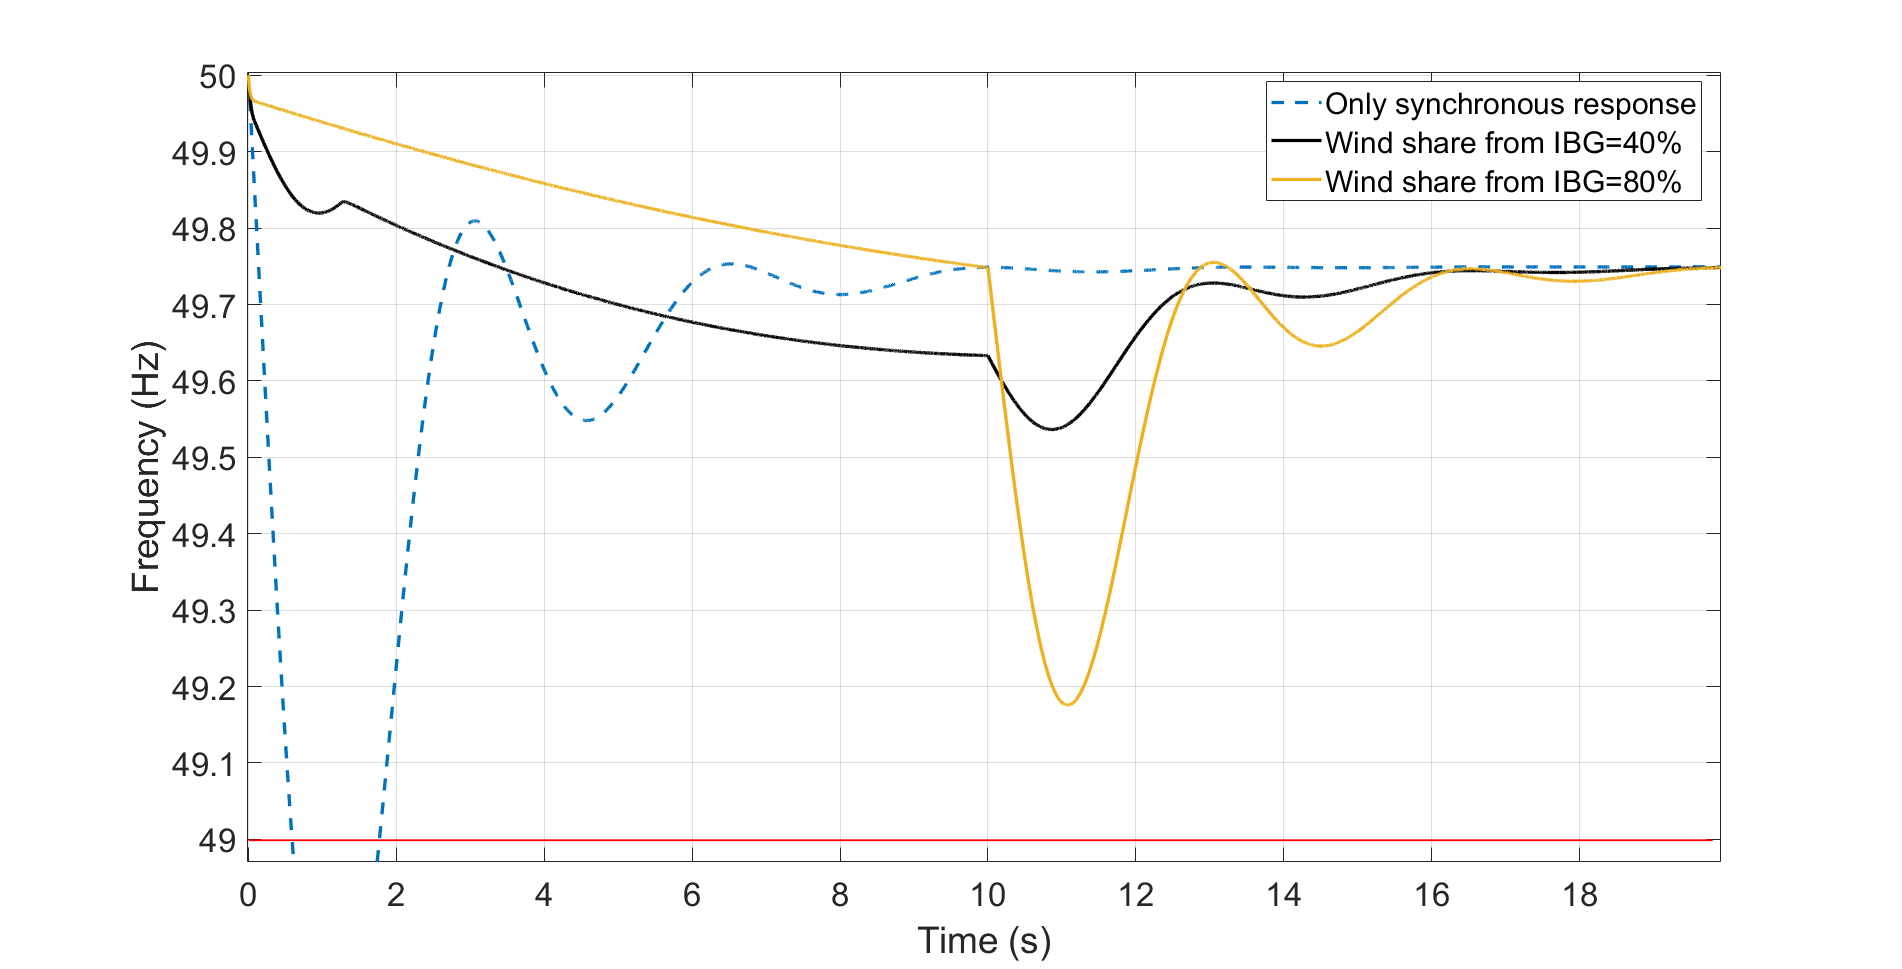
\includegraphics[width=\textwidth]{result/SI10imb}
		\caption{}
		\label{fig:res_ieee_fr10imb}
	\end{subfigure}
	\hfill
	\begin{subfigure}[h]{0.49\textwidth}
		\centering
		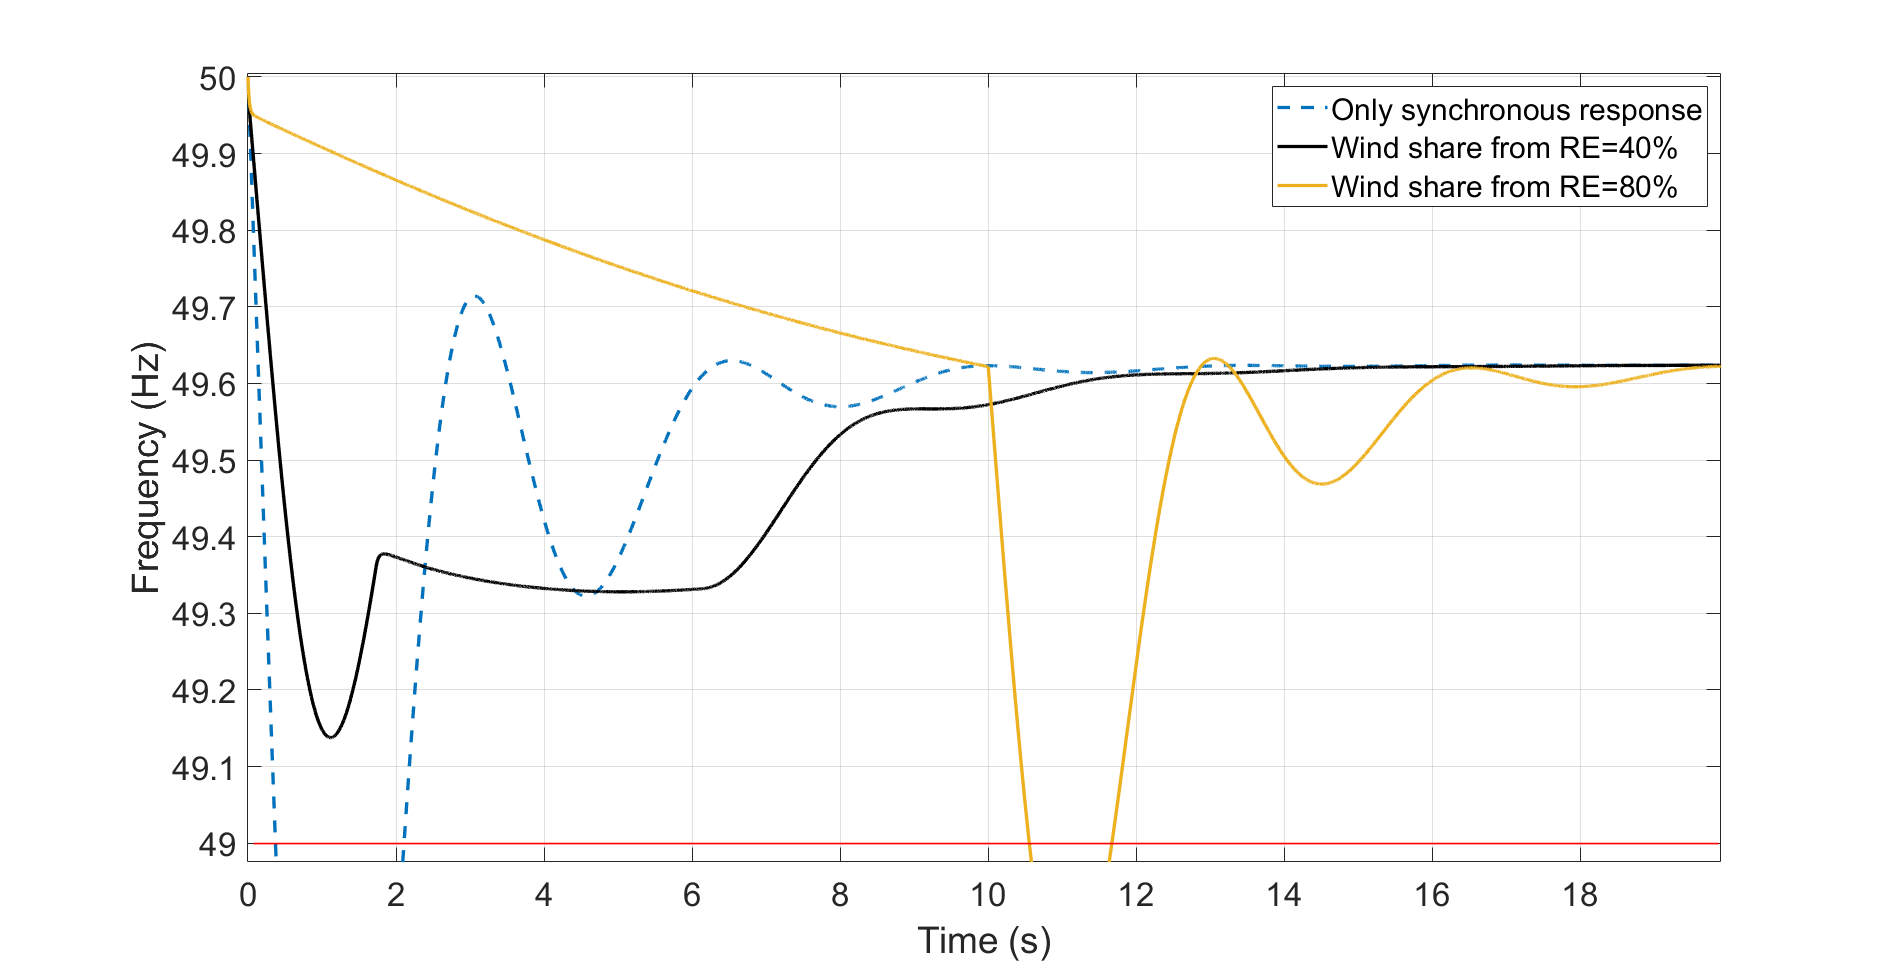
\includegraphics[width=\textwidth]{result/SI15imb}
		\caption{}
		\label{fig:res_ieee_fr15imb}
	\end{subfigure}
	\caption{Frequency response is presented for an imbalance of 10\% in (\textbf{a}) and 15\% in (\textbf{b}). Cases with contribution of 40\% and 80\% of the total IBG share are compared with the scenario with no support coming from IBG.}
\end{figure}

\subsubsection{Effect of Power Ramp Response on Frequency}

The contribution from the ramping power in diminishing system RoCoF from the inception of the perturbation until the critical time was disregarded when Equation \eqref{eq:p_at_tcr} was calculated. Assuming an instant switching of the IBFPR at critical time, the frequency nadir would be 49 Hz. Nevertheless, a ramp power response was assumed instead. Therefore the frequency response of a unbalanced system, commonly exhibits a frequency nadir higher than 49 Hz due to the contribution of the ramping period. In this sense, it can be inferred that the longer the ramping period, the higher frequency nadir will be obtained. Here again the relevance of the prompt activation in time of the IBFPR. On the other hand, with the faster activation of IBFPR, the ramp slope and the steady power output can be diminished compromising frequency nadir.\\ 

When a comparison is established bewteen all the calculated power ramp slopes in per unit (pu), it can be noticed that with a high penetration of non-synchronous power in the system, the required power to ensure no UFLS have a consistent trend between the three models and a close proximity. This in the values for RoCoF in the range of 2 to 5 Hz/s. Such trends can be seen in \ref{fig:res_pramp}. A bigger amount of power ramp slope is needed in all the range of RoCoF for the European case. After inspecting Equation \ref{eq:IBFPR}, it is noticed that the IBFPR is affected by the factor $ 1-t_{cr} /t_{nadir} $, then as nadir time increases, IBFPR increases as well. The nadir time for the European case, due to the action of the self-regulation and primary reserve deployment of 30 seconds, is in the range of 3-12 seconds (6 seconds for 80\% IBG penetration) whereas the nadir time for the simplified IEEE model is between 1-3 seconds.\\

\begin{figure}[h]
	\centering
	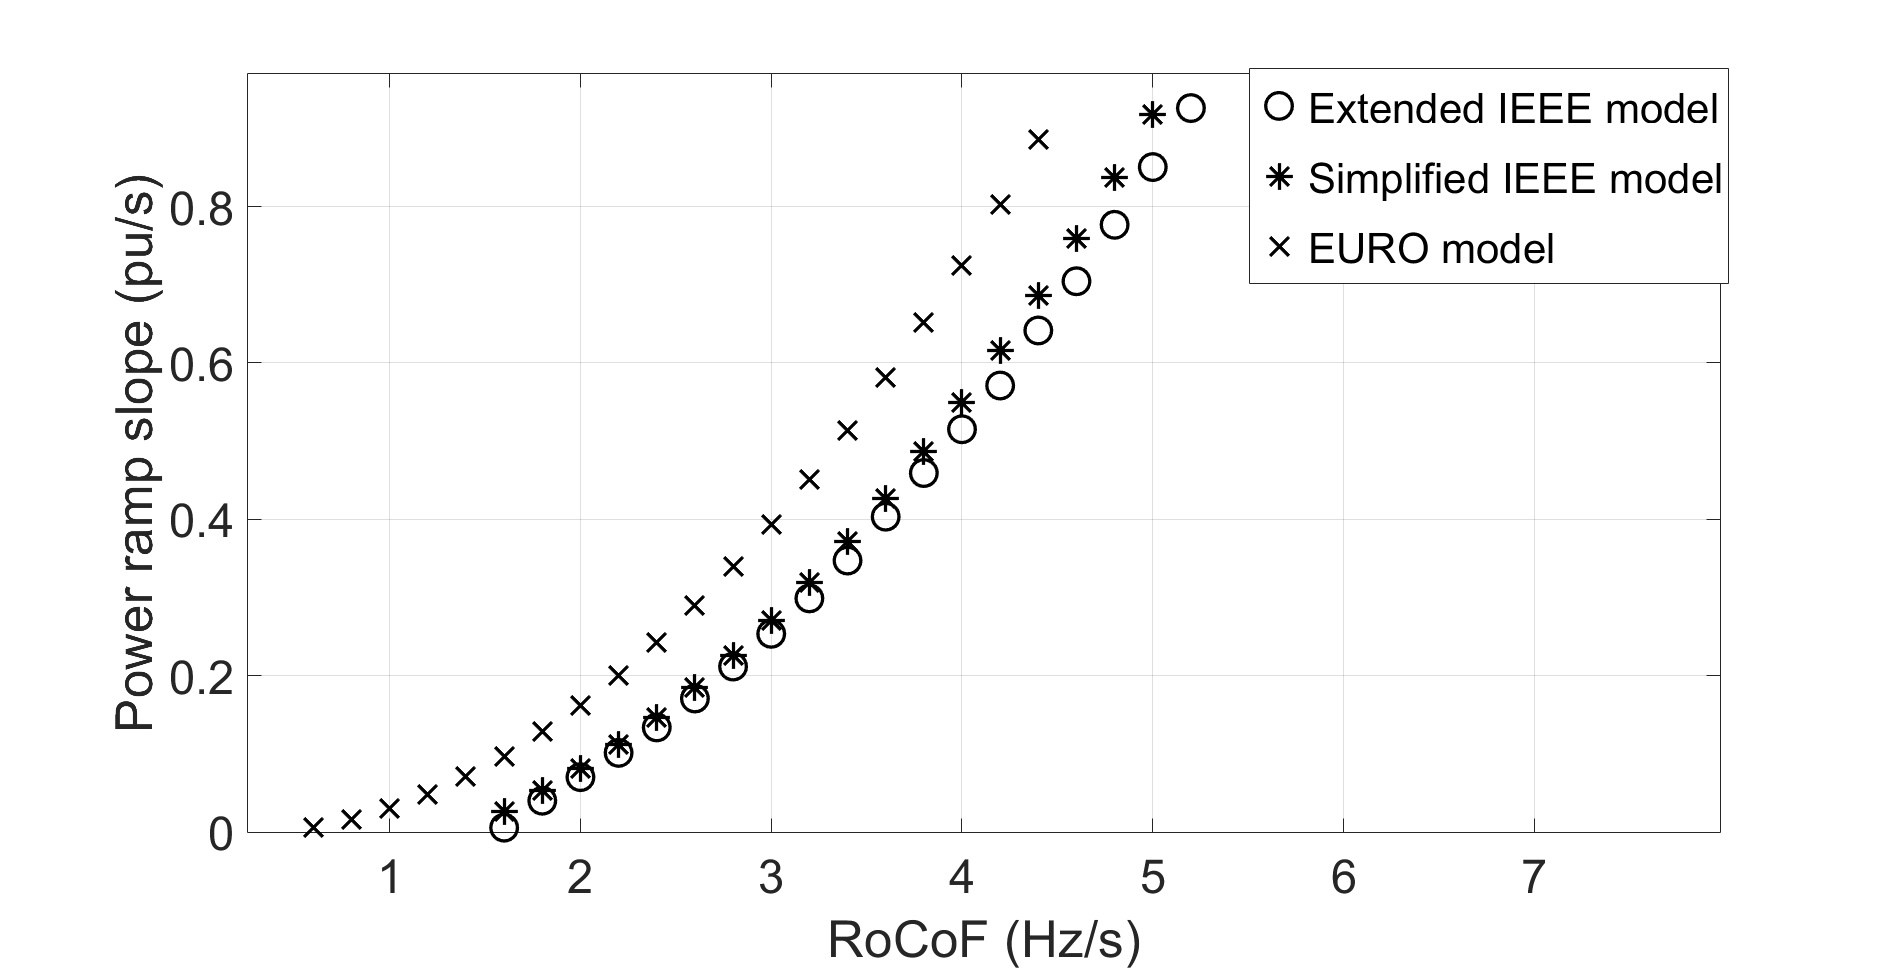
\includegraphics[width=0.75\textwidth]{/result/powerramps}
	\caption{Comparison of the results of the three models in terms of the IBFPR power ramp which is needed at 80\% of share from non-synchronous generation.}
	\label{fig:res_pramp}
\end{figure}

\subsubsection{Fast Power Reserve}


The required power ramp  to avoid load shedding has been found for both IEEE 9 bus models with a fast governor response and for the European-scale model  with conventional primary reserve response. Hence, the IBFPR at critical time which remain constant after the critical time, would be accounted as the fast power reserve. In Table \ref{tb:crpowr} the required values for the inverter base reserve for the European model are listed for imbalances out of the dimmensioning case of ENTSOE.

\begin{table}[h]
	\caption{\label{tb:crpowr}: Fast power reserve in per unit for the European case. Power reserve expressed in pu with power load as the base}
	\centering
	%% \tablesize{} %% You can specify the fontsize here, e.g., \tablesize{\footnotesize}. If commented out \small will be used.
	\begin{tabular}{*9c}
		\toprule
		\textbf{IBG share (\%)}	& \multicolumn{8}{c}{\textbf{Load Imbalance (\%)}} \\
		\midrule
		{} & 3&	4&	5&	6&	7&	8&	9	&10 \\
		\midrule
		20&	-&	-&	0.025&	0.038&	0.049&	0.060&	0.070&	0.081\\
		40&	-&	0.016&	0.030&	0.041&	0.052&	0.063&	0.073&	0.083\\
		60&	0.005&	0.024&	0.035&	0.045&	0.056&	0.066&	0.077&	0.087\\
		80&	0.016&	0.028&	0.039&	0.049&	0.062&	0.070&	0.080&	0.09\\
		92&	0.021&	0.033&	0.043&	0.054&	0.064&	0.074&	0.084&	0.094\\
		95&	0.024&	0.035&	0.045&	0.055&	0.065&	0.075&	0.085&	0.096\\
		\bottomrule
	\end{tabular}
\end{table}

When IBFPR is implemented in all three cases, frequency drop below 49Hz is avoided for almost all values of RoCoF, provided that enough IBFPR is available for the given imbalance. Figures \ref{fig:res_ieee_ibfpr} to \ref{fig:res_euro_ibfpr} show the frequency nadir for all the cases.\\

\begin{figure}[h]
	\centering
	\begin{subfigure}[h]{0.49\textwidth}
		\centering
		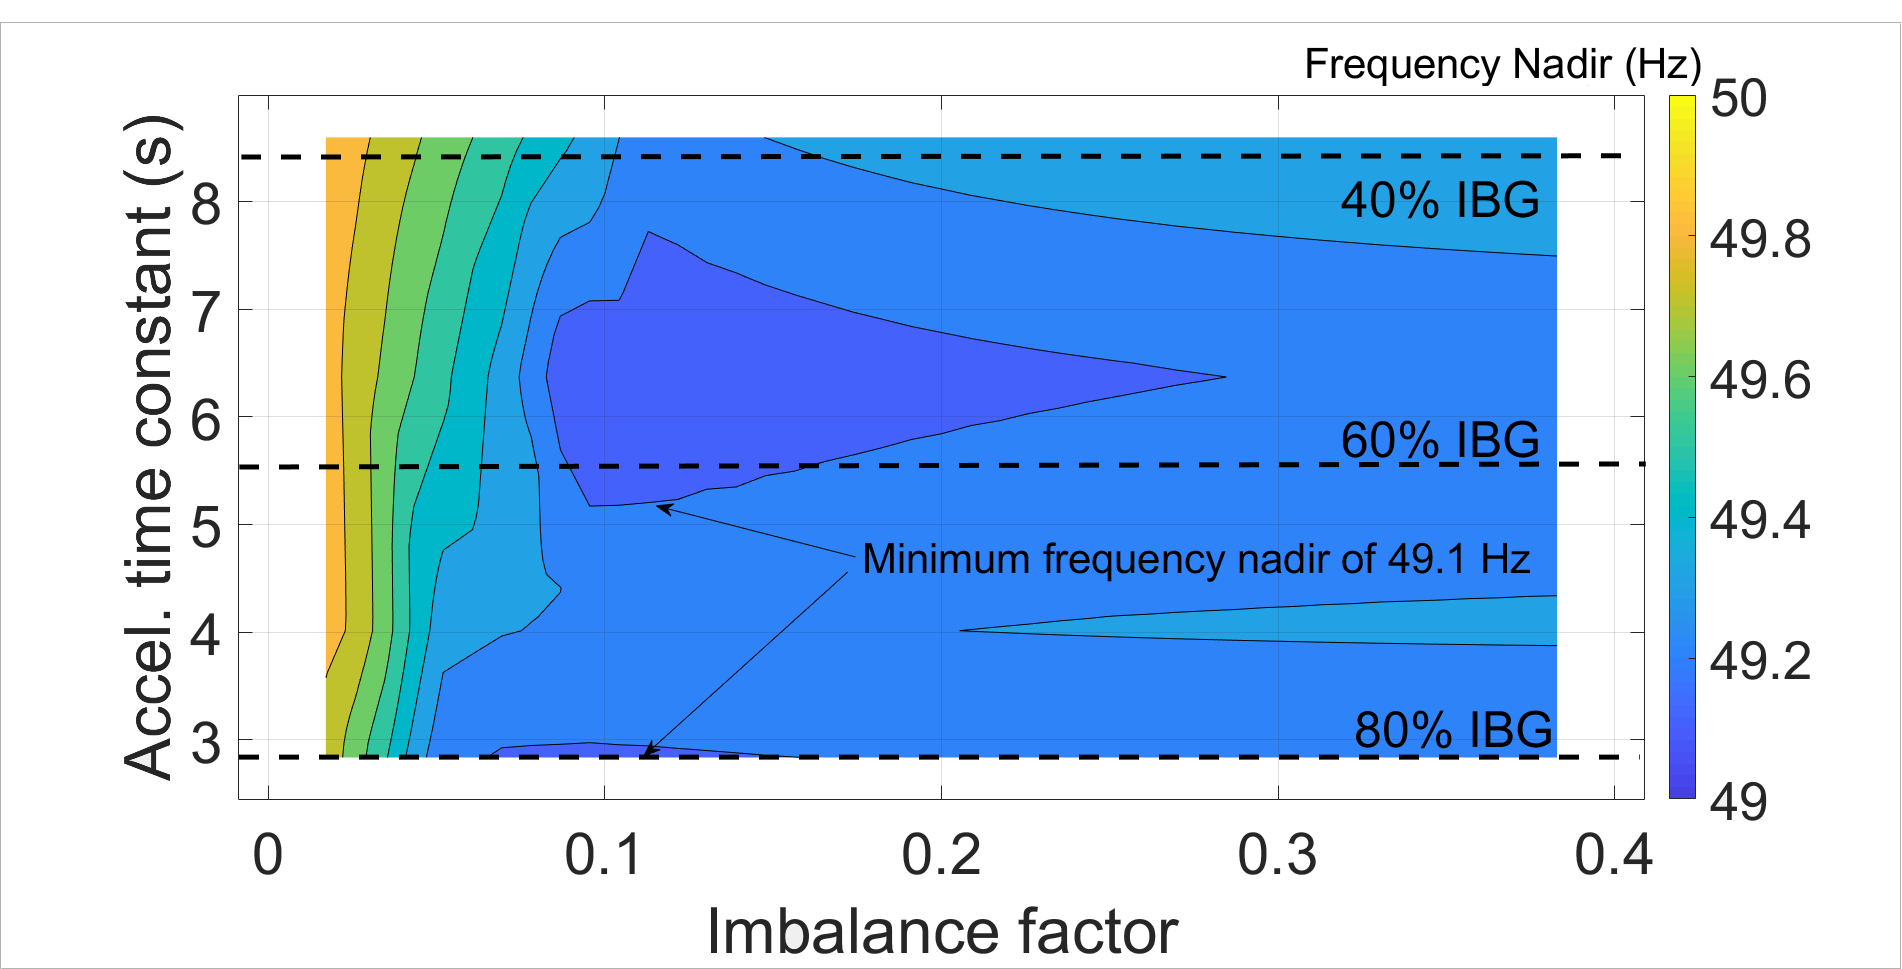
\includegraphics[width=\textwidth]{result/NadirIBFPR2}
		\caption{}
		\label{fig:res_ieee_ibfpr}
	\end{subfigure}
	\hfill
	\begin{subfigure}[h]{0.49\textwidth}
		\centering
		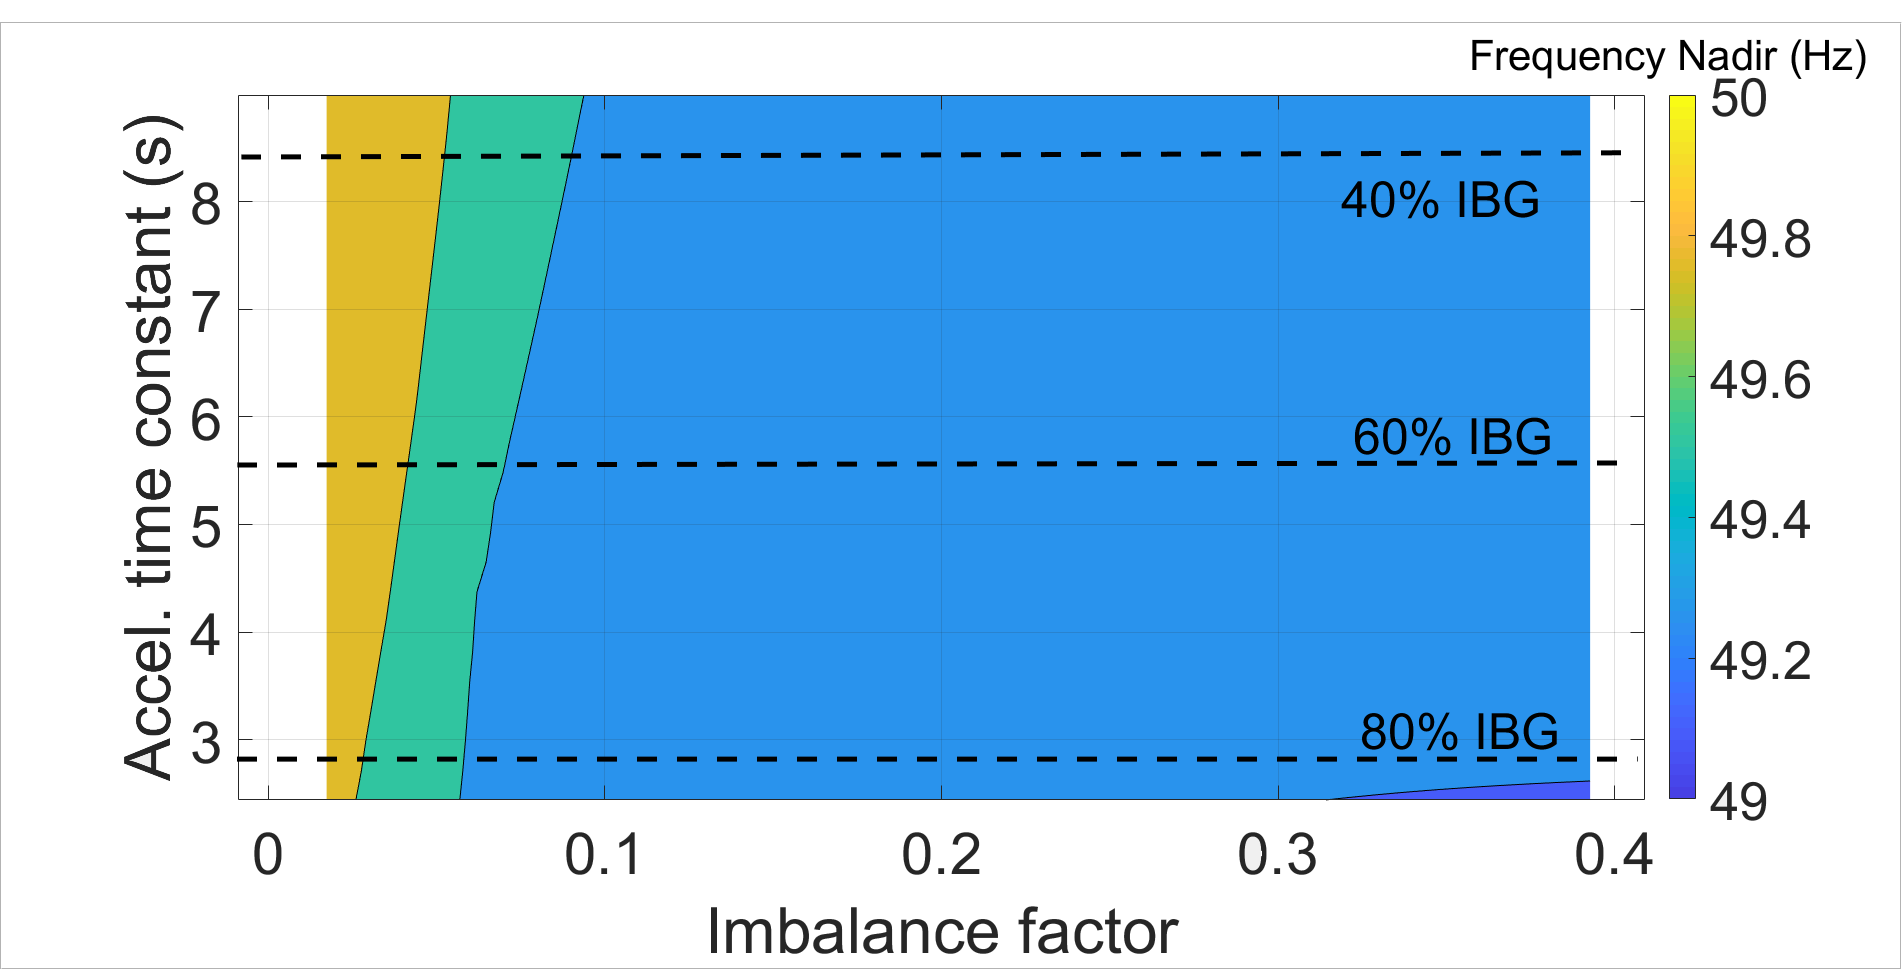
\includegraphics[width=\textwidth]{result/extnd}
		\caption{}
		\label{fig:res_extd_ibfpr}
	\end{subfigure}
	\hfill
	\begin{subfigure}[h]{0.49\textwidth}
		\centering
		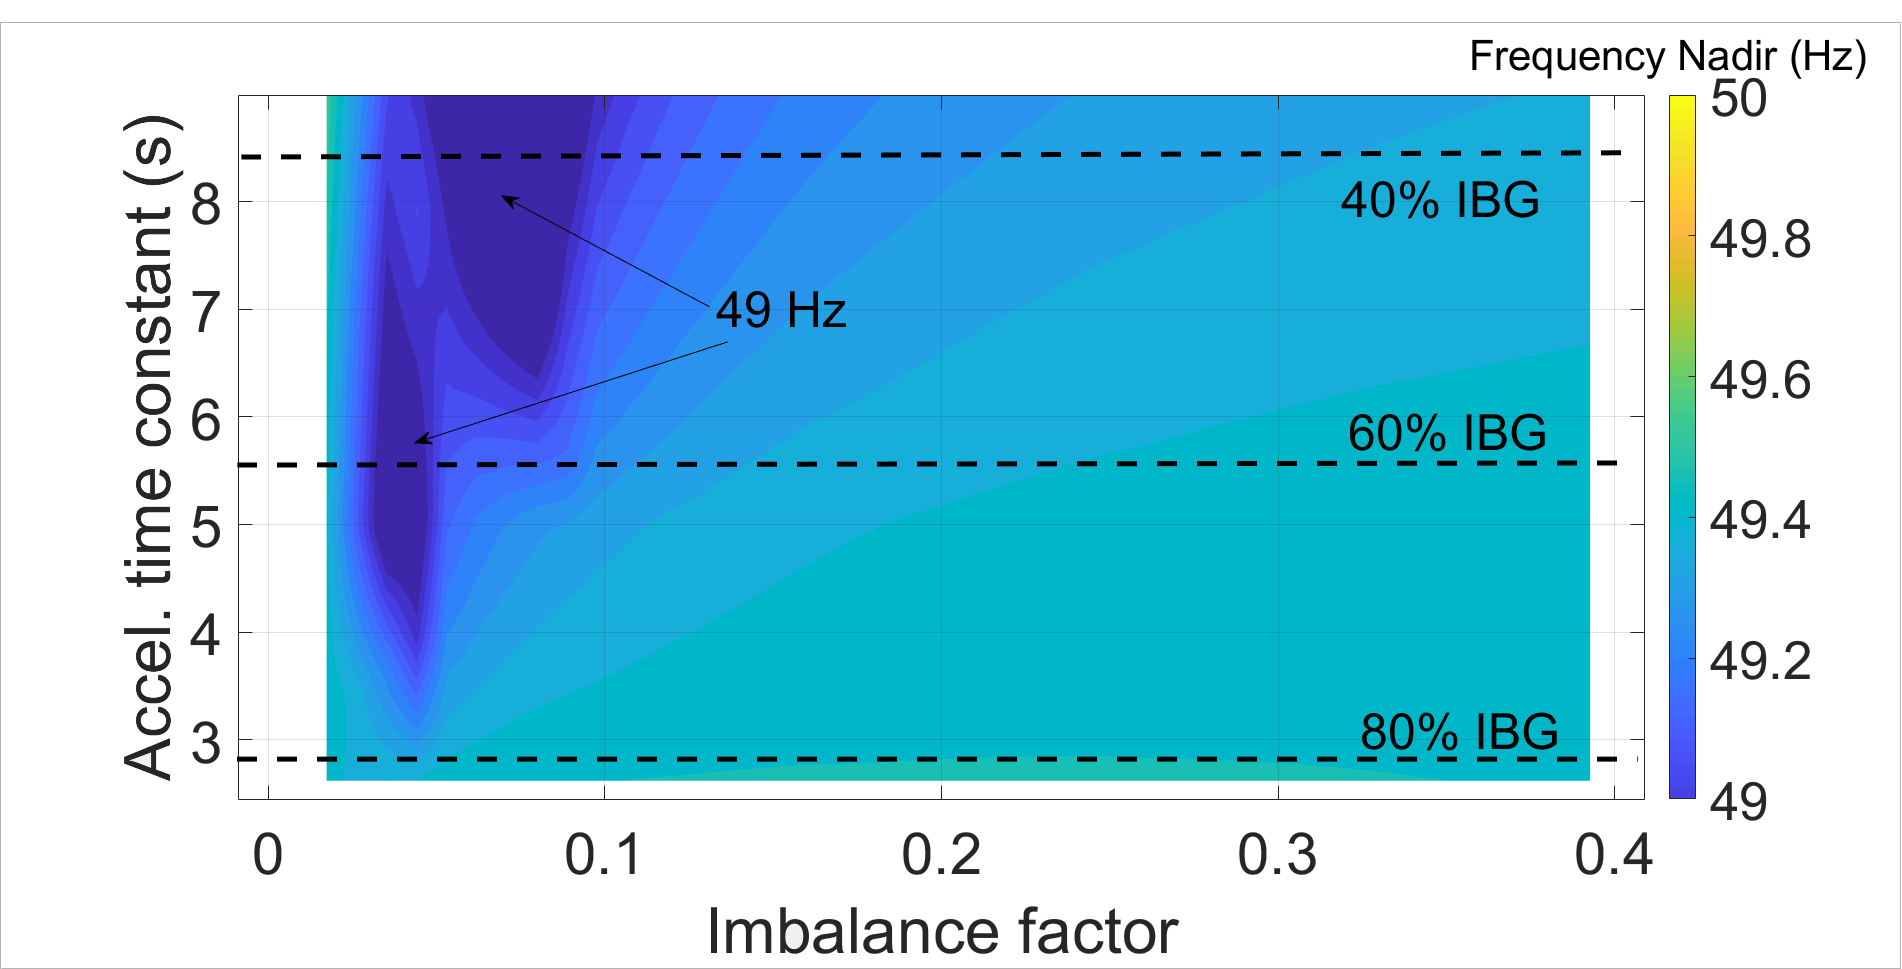
\includegraphics[width=\textwidth]{result/eu}
		\caption{}
		\label{fig:res_euro_ibfpr}
	\end{subfigure}
	
	
	\caption{Frequency nadir with the implementation of IBFPR in: (\textbf{a}) The simplified IEEE model  (\textbf{b}) The extended IEEE model. (\textbf{c}) The large scale (European model). }
\end{figure}
%For imbalances higher than 3\% the fast power reserve has to cover mostly all the imbalance. The observed offset from the one to one relation is due to the load reduction caused by the frequency drop (load self-regulation). The dashed line represents the one to one proportion. In the case of the IEEE grid; the simplified model exhibits a permanent offset from the dashed line of around 0.05 pu, this due to the action of a faster governor response. Therefore, it can be said that in such scenario, the conventional governor response of synchronous machines would cover 5\% of the imbalances starting at 8\%. Since the values for nadir time are not independent from the imbalance in the Extended model, due to the non-linearity of the model, the calculated power reserve tend to equalize the whole imbalance. As imbalance increases, the critical time decreases and the nadir time increases, this makes the reducing factor tcr/tnadir from Equation 3-2 to decrease and narrows the difference between the calculated reserve and power imbalance.
%Similarly as critical time was presented in Table 5 1 the required fast power reserve in the European context is shown in Table 5 2 for extraordinary events


%As IBG increases the closer to the imbalance the fast power reserve needs to be. As it was demonstrated in the result section; with a faster conventional reserve, reduction in fast power reserve can be observed.

\subsection{Synchronizing effect, lack of damping torque and implications}

The diminishing of synchronous machines in the system leads to a very weak network where synchronizing and damping torque, which are inherent characteristics of synchronous machines, are not enough to stabilize the system[7]. Although the implementation of IBFPR contributes keeping synchronous machine on step, oscillations in the speed/frequency response of the rotor are observed. Figure XXX show the speed of the rotor machines after a perturbation and power balancing through the implementation of IBFPR in the IEEE extended model. This oscillations are created by the lack of damping torque which is provided mainly by the synchronous machines through damping windings, rotor field exciter and power system stabilizer[ref]. \\

\begin{figure}[h]
	\centering
	\begin{subfigure}[h]{0.49\textwidth}
		\centering
		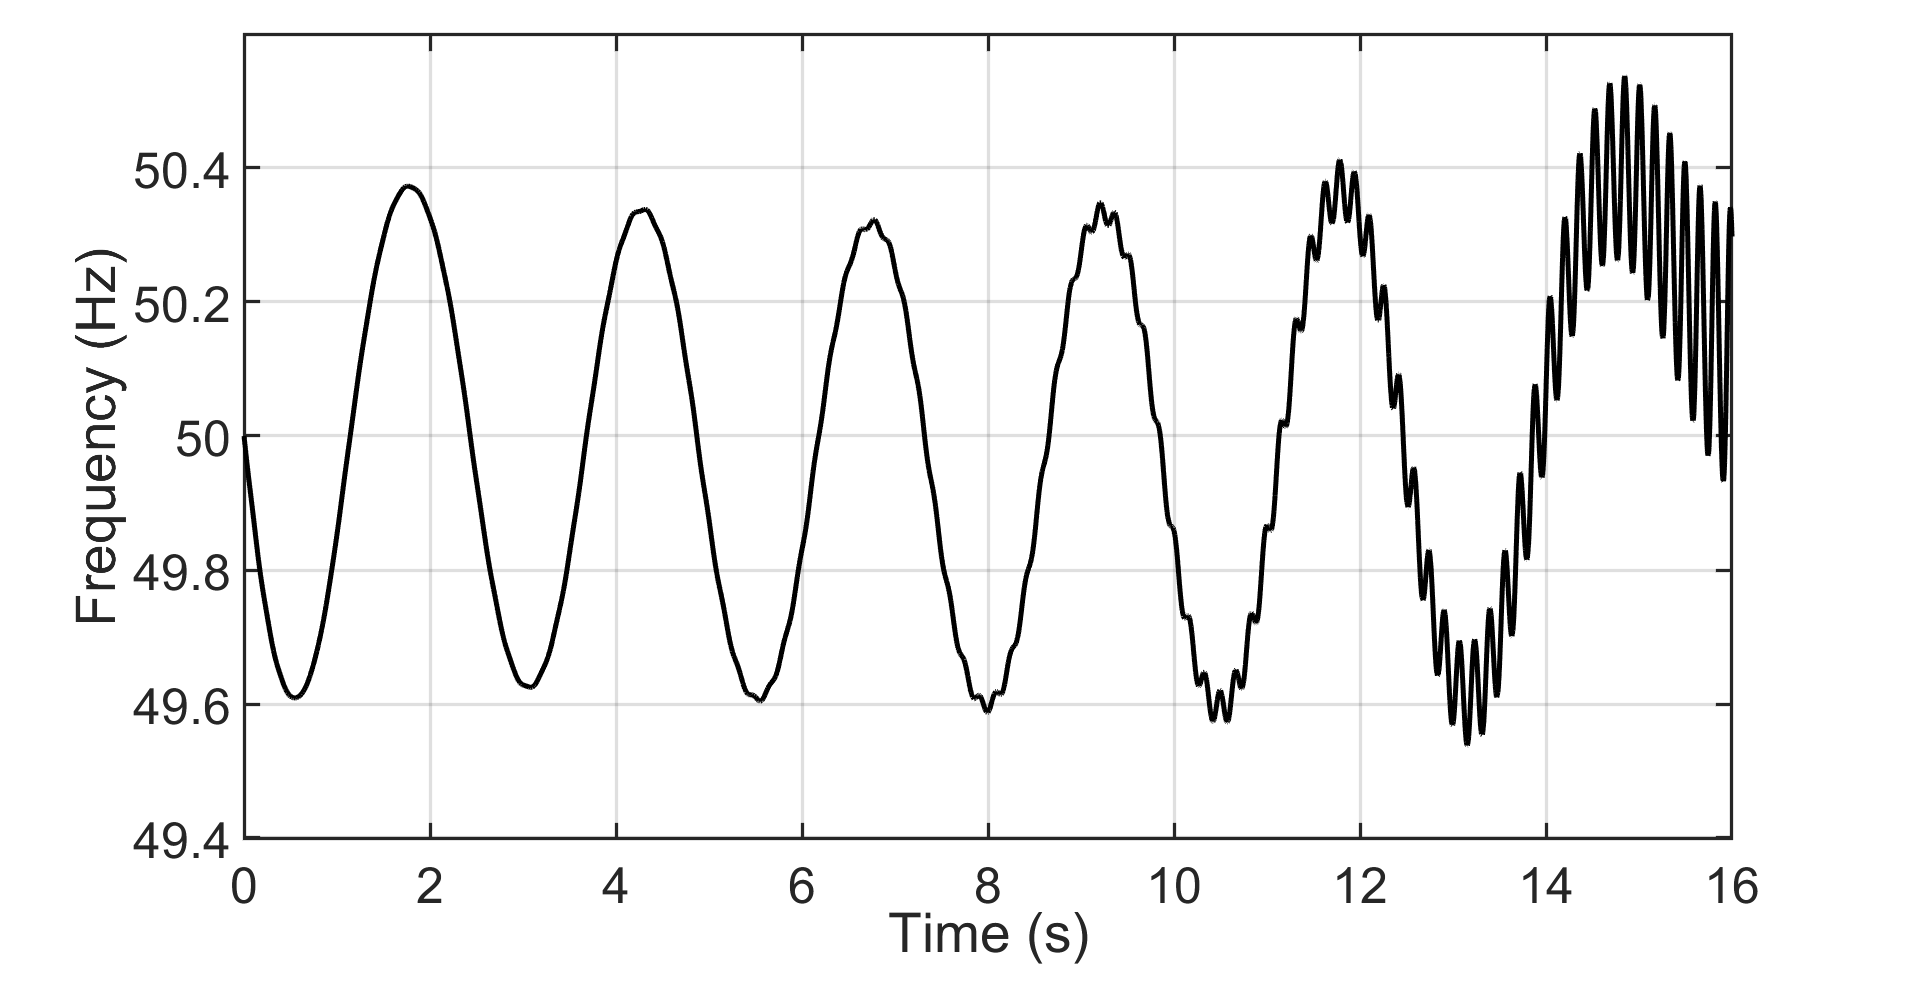
\includegraphics[width=\textwidth]{result/ss1}
		\caption{}
		\label{fig:res_osc_noIBFPR}
	\end{subfigure}
	\hfill
	\begin{subfigure}[h]{0.49\textwidth}
		\centering
		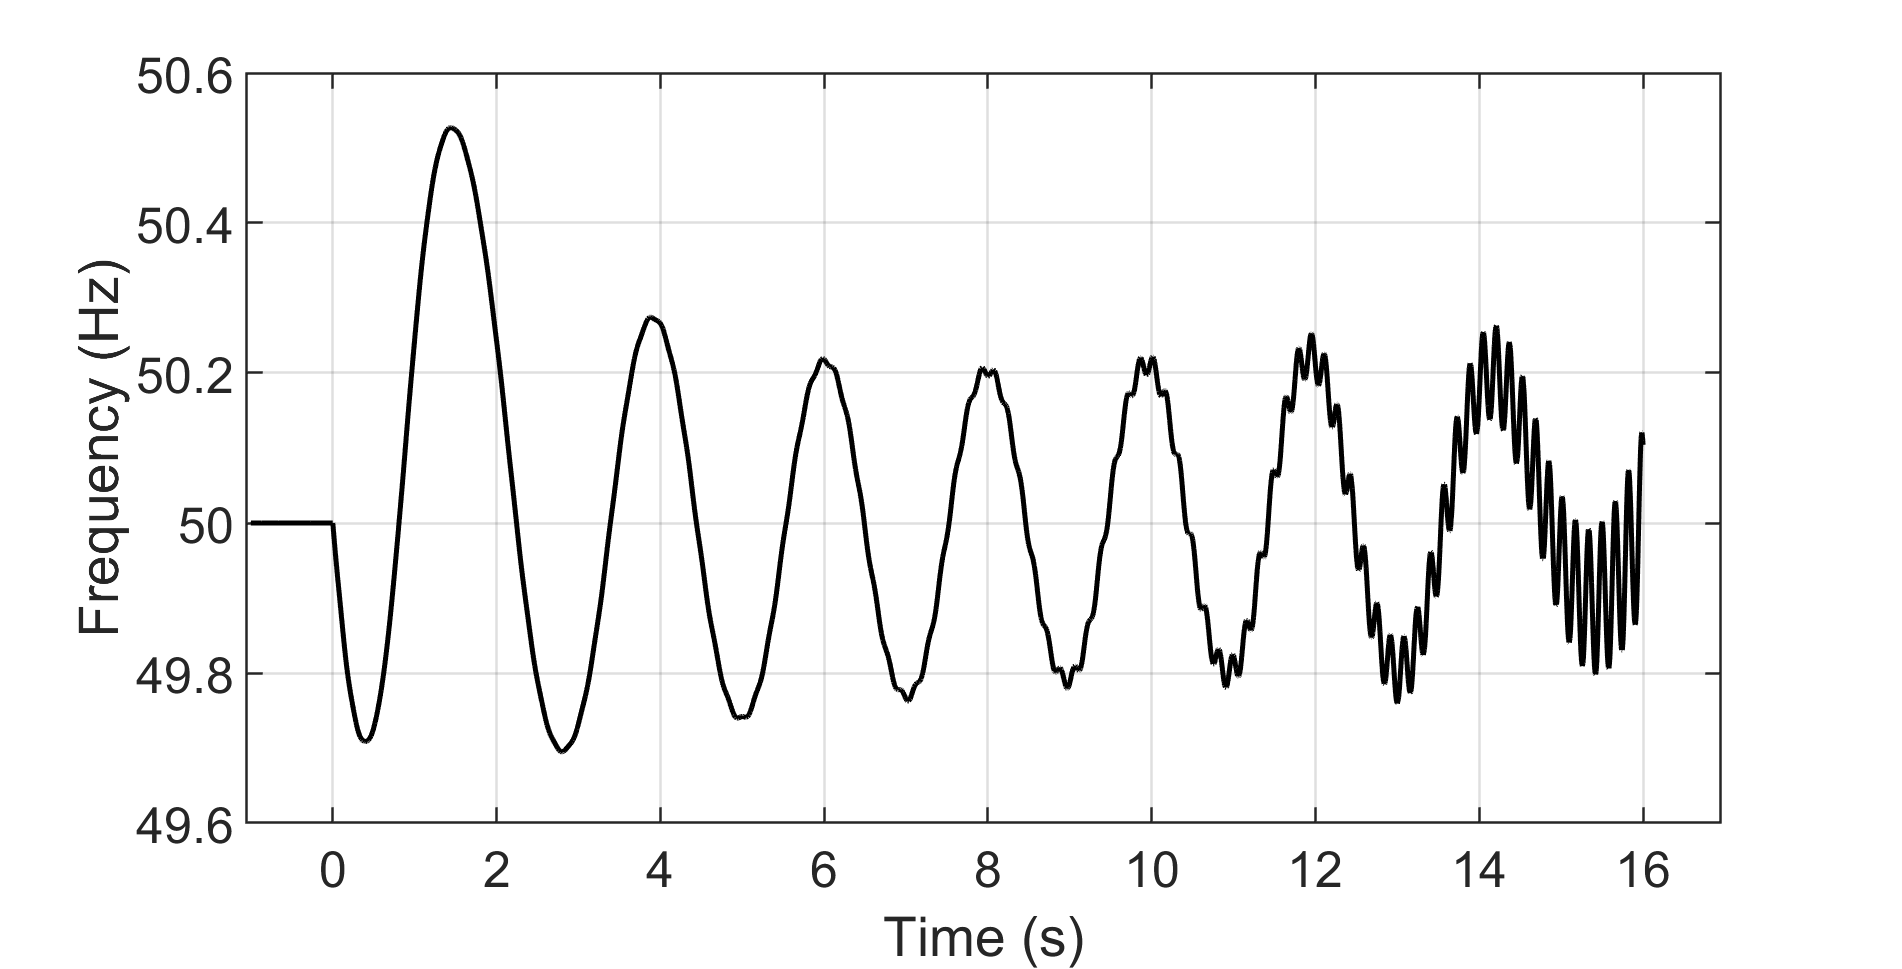
\includegraphics[width=\textwidth]{result/ss2}
		\caption{}
		\label{fig:res_osc_IBFPR}
	\end{subfigure}
	
	
	\caption{In (\textbf{a}) the oscillatory frequency response is depicted when no additional frequency support is given by the IBG, whereas in  (\textbf{b}) the IBFPR is applied. In both cases an imbalance of 2\% and a penetration of 95\% of IBG were considered.}
\end{figure}

%Discussion
%For the simplified IEEE model and the European island, only transfer functions describing an equivalent system governor were modeled. Hence in such approaches, the effect and dynamics of synchronous generator’s exciters and inter-machine interaction were not taken into account. The before mention factors influence greatly small signal stability [7, 8]
%Even though the scoop of this thesis is to analyze the power-time characteristics needed to avoid frequency collapse; oscillations associated to big perturbation were observed but they could not been addressed by the simple injection of power to the system. Also in the IEEE model, when a penetration of 95\% of inverter based generation and 2\% of load imbalance are considered, UFLS is not reached but the system becomes unstable as shown in Figure 5 6 and Figure 5 5. From penetrations levels above 85\% complete frequency stability is not ensure with the injection of fast power reserve, only UFLS on the first 10 seconds approximately. Then the system becomes unstable with increasing amplitude oscillations.
%It is important to note that ENTSOE in its EUROPEAN interconnected scenario, determined that there is no UFLS when an unbalance of 2\% with high contribution of non-synchronous generation occurs. Nevertheless, no inter-machine interaction was considered and therefore a similar effect as the one in Figure 5 6 could be experienced.%Discussion
